%%%%%%%%%%%%%%%%%%%%%%%%%%%%%%%%%%%%%%%%%%%%%%%%%%%%%%%%%%%%%%%%%%%%%%
% Séquence « Limites et continuité » — fichier commun aux deux versions.
% Texte du cours : séquences/limite_continuite.tex (I.L. TASSIGUI).
% Ajouts : environnements corrige, preuve, noteprof (voir outils_versions.tex).
% Les blocs \resultat sont réservés à la version enseignant.
%%%%%%%%%%%%%%%%%%%%%%%%%%%%%%%%%%%%%%%%%%%%%%%%%%%%%%%%%%%%%%%%%%%%%%
\section{Limites et continuité}
\activity{Rappels sur les limites}{1}{
 Désemparé  par les  résultats  des deux devins, Dansou décide de se consacrer à ses études pour réussir à son examen. Cependant, il a quelques difficultés dans le calcul des limites. Tu vas l'aider en te basant sur tes connaissances antérieures, pour résoudre les consignes de cette séquence.
}
\begin{noteprof}
Cette séquence s'appuie sur les acquis de Première (limites, opérations, asymptotes). On peut commencer par un rappel oral rapide des limites usuelles avant d'aborder la consigne 1.1, puis consacrer l'essentiel du temps à la continuité, au théorème des valeurs intermédiaires et aux bijections, qui sont nouveaux.
\end{noteprof}
\ifenseignant % --- cours (absent de la version élève) ---
\subsection{Limites de fonctions usuelles}
Soit $k\in \R$, et $n$ un entier naturel non nul.
\begin{boite}
	\begin{multicols}{2}
		\item[$\bullet$] \limite{x}{-\infty}{k=k} et \limite{x}{+\infty}{k=k}
		\item[$\bullet$] \limite{x}{+\infty}{\sqrt{x}=+\infty}
		\item[$\bullet$] \limite{x}{+\infty}{x^n=+\infty}
		\item[$\bullet$] \limite{x}{-\infty}{x^n =
			\begin{cases}
				+\infty \text{, si }n\text{ est pair.}\\
				-\infty\text{, si }n\text{ est impair.}
			\end{cases}
		}
		\item[$\bullet$] \limite{x}{-\infty }{\f{1}{x^n}=0} et  \limite{x}{+\infty }{\f{1}{x^n}=0}
		\item[$\bullet$] \limite{x}{0}{\f{\sin x}{x}=1}\\ \item[$\bullet$]\limite{x}{0}{\f{\tan x}{x}=1}\\
		\item[$\bullet$] \limite{x}{0}{\f{\cos x -1}{x}=0}\\
		\item[$\bullet$] \limite{x}{0}{\f{1-\cos x}{x^2}=\f{1}{2}}
	\end{multicols}
\end{boite}
\begin{preuve}
La limite \limite{x}{0}{\f{\sin x}{x}=1} est admise (elle s'obtient géométriquement à partir de l'encadrement $\cos x\leq \f{\sin x}{x}\leq 1$ pour $x\in\intervOO{0}{\f{\pi}{2}}$). On en déduit les trois autres :
\begin{itemize}
	\item $\f{\tan x}{x}=\f{\sin x}{x}\times\f{1}{\cos x}$, donc \limite{x}{0}{\f{\tan x}{x}=1\times 1=1}.
	\item $\f{1-\cos x}{x^2}=\f{1-\cos^2 x}{x^2(1+\cos x)}=\bigg(\f{\sin x}{x}\bigg)^2\times\f{1}{1+\cos x}$, donc \limite{x}{0}{\f{1-\cos x}{x^2}=1\times\f{1}{2}=\f{1}{2}}.
	\item $\f{\cos x-1}{x}=-x\times\f{1-\cos x}{x^2}$, donc \limite{x}{0}{\f{\cos x-1}{x}=0\times\f{1}{2}=0}.
\end{itemize}
\end{preuve}
\subsection{Opérations algébriques}
\fi % --- fin cours ---
\begin{acoller}{Opérations sur les limites}
Soient $f$ et $g$ deux fonctions numériques telles que $D_f\cap D_g\neq \emptyset$. $x_0$ est un réel, ou égal à $-\infty$, ou à $+\infty$, au voisinage duquel $f$ et $g$ sont définies.
{\newcolumntype{Y}{>{\raggedleft\arraybackslash}X}% see tabularx
	\tcbset{enhanced,fonttitle=\bfseries\large,
		colback=yellow!10!white,colframe=red!50!black,colbacktitle=green!30!white,
		coltitle=black,center title}
	\begin{tcolorbox}[tabularx={p{2.3cm}|p{1.8cm}||p{0.7cm}||p{3cm}|p{3cm}|X},title=Opérations sur les limites,sharp corners]
		Si \limite{x}{x_0}{f(x)=} & \limite{x}{x_0}{g(x)=}	& alors	& \limite{x}{x_0}{\big(f+g\big)(x)=}	& 	\limite{x}{x_0}{\big(f\times g\big)(x)=}& \limite{x}{x_0}{\bigg(\f{f}{g}\bigg)(x)=}\\\hline\hline
		\centering$\ell$	& \centering$\ell '$ &  &\centering $\ell +\ell '$& \centering$\ell\times \ell'$ &$\begin{cases}
		\f{\ell}{\ell'}\text{; si }\ell\neq 0\text{ et }\ell'\neq 0\\
		0\text{; si }\ell=0\text{ et }\ell'\neq 0\\
		\pm\infty\text{; si }\ell \neq 0\text{, }\ell'=0^\pm
		\end{cases}$\\\hline
		\centering$0$&\centering$0$&&\centering$0$&\centering$0$&\textbf{On ne peut pas conclure}\\\hline
		\centering$\ell \neq 0$&\centering$\pm\infty$&&\centering$\pm\infty$&$\begin{cases}
		\pm\infty\text{; si }\ell>0\\
		\mp\infty\text{; si }\ell<0
		\end{cases}$&$0$\\\hline
		\centering$0$&\centering$\pm\infty$& &\centering$\pm\infty$&\textbf{On ne peut pas conclure}&$0$\\\hline

		\centering$\pm\infty$&\centering$\ell'\neq 0$& &\centering$\pm\infty$&$\begin{cases}
		\pm\infty\text{; si }\ell'>0\\
		\mp\infty\text{; si }\ell'<0
		\end{cases}$&$\begin{cases}
		\pm\infty\text{; si }\ell'>0\\
		\mp\infty\text{; si }\ell'<0
		\end{cases}$\\\hline
		\centering$\pm\infty$&\centering$ 0$& &\centering$\pm\infty$&\textbf{On ne peut pas conclure}&$\begin{cases}
		\pm\infty\text{; si }0^+\\
		\mp\infty\text{; si }0^-
		\end{cases}$\\\hline
		\centering$\pm\infty$&\centering$\pm\infty$& &\centering$\pm\infty$&\centering$+\infty$&\textbf{On ne peut pas conclure}\\\hline
		\centering$\pm\infty$&\centering$\mp\infty$& &\textbf{On ne peut pas conclure}&\centering$-\infty$&\textbf{On ne peut pas conclure}\\\hline
\end{tcolorbox}}
\begin{noteprof}
Dans la ligne « $\pm\infty$ et $0$ » du quotient, le fichier d'origine indiquait deux fois « $\pm\infty$ si $0^\pm$ » ; la deuxième ligne a été corrigée en « $\mp\infty$ si $0^-$ ». Insister sur le fait que le signe de la limite d'un quotient dépend du signe de $0$ ($0^+$ ou $0^-$) : faire systématiquement un tableau de signes du dénominateur.
\end{noteprof}
%\begin{remarque}
%\subsection{Formes indéterminées}
Les cas où on ne peut pas conclure sont les formes indéterminées. Ce sont les cas : \og $-\infty+(+\infty)$\fg{ }; \og $0\times \infty$\fg{ }; \og $\f{0}{0}$\fg{ } et \og $\f{\infty}{\infty}$\fg{ }. Ils nécessitent des transformations appropriées (factorisation, expression conjuguée, division euclidienne \dots)
\begin{remark}
	\begin{itemize}
		\item[\ding{182}] La limite en l'infini d'une fonction polynôme est égale à la limite de son monôme de plus haut degré.
		\item[\ding{183}] La limite à l’infini d’une fonction rationnelle est égale à la limite à l’infini du
		quotient simplifié de ses termes de plus hauts degrés.
	\end{itemize}
\end{remark}
\begin{preuve}
\ding{182} Si $P(x)=a_nx^n+\dots+a_1x+a_0$ avec $a_n\neq 0$, alors pour $x\neq 0$ : $P(x)=a_nx^n\bigg(1+\f{a_{n-1}}{a_nx}+\dots+\f{a_0}{a_nx^n}\bigg)$. La parenthèse tend vers $1$ en l'infini, donc $P(x)$ a la même limite que $a_nx^n$.
\par \ding{183} On factorise de même le numérateur et le dénominateur par leurs monômes de plus haut degré.
\end{preuve}
\end{acoller}
\begin{acoller}{Lever une forme indéterminée}
\begin{center}
% Organigramme : lever une forme indéterminée (remplace images/forme_ind.jpg)
\begin{tikzpicture}[
	font=\small,
	>=latex,
	titre/.style={draw,thick,rounded corners=2pt,fill=#1,inner sep=5pt,font=\normalsize\bfseries},
	cas/.style={draw,fill=#1,inner sep=4pt,align=center},
	boite/.style={draw,fill=#1,inner sep=5pt,align=left},
	fl/.style={->,thick},
	]
	\node[text width=17cm,align=left] (obj) at (0,0) {L'objectif est de calculer \limite{x}{a}{f(x)}, où $a$ représente un réel, $+\infty$ ou $-\infty$.};
	%%%%%%%%%%%%%%%%%%%% Forme infini / infini %%%%%%%%%%%%%%%%%%%%
	\node[titre=green!15] (T1) at (0,-1.1) {Forme indéterminée \og $\f{\infty}{\infty}$\fg{}};
	\node[cas=orange!15,text width=6.5cm] (A1) at (-4.6,-2.3) {\bfseries Les fonctions rationnelles};
	\node[cas=orange!15,text width=6.5cm] (B1) at (4.6,-2.3) {\bfseries $f(x)$ contient une racine carrée};
	\node[boite=white,text width=7.6cm,anchor=north] (A2) at ([yshift=-0.25cm]A1.south) {La limite en $+\infty$ (ou en $-\infty$) d'une fonction rationnelle est égale à la limite du quotient de ses termes de plus haut degré au numérateur et au dénominateur.};
	\node[boite=white,text width=7.6cm,anchor=north] (B2) at ([yshift=-0.25cm]B1.south) {On met le terme de plus haut degré en facteur sous la racine ($x\neq 0$) :\\[1mm]
		\centering $\sqrt{ax^2+bx+c}=\lvert x\rvert\sqrt{a+\f{b}{x}+\f{c}{x^2}}$\par\smallskip $\sqrt{ax+b}=\lvert x\rvert\sqrt{\f{a}{x}+\f{b}{x^2}}$};
	\draw[fl] (T1.west) -| (A1.north);
	\draw[fl] (T1.east) -| (B1.north);
	%%%%%%%%%%%%%%%%%%%% Forme +infini - infini %%%%%%%%%%%%%%%%%%%%
	\node[titre=cyan!15] (T2) at (0,-6.1) {Forme indéterminée \og $+\infty-\infty$\fg{}};
	\node[cas=yellow!20] (R) at (0,-7.2) {\bfseries $f(x)$ contient une racine carrée};
	\node[cas=magenta!15,text width=4.3cm] (C1) at (-6.4,-8.5) {$f(x)=\sqrt{ax+b}+\alpha x+\beta$};
	\node[cas=magenta!15,text width=5.6cm] (C2) at (-0.6,-8.5) {$f(x)=\sqrt{ax^2+bx+c}-\sqrt{\alpha x^2+\beta x+\delta}$};
	\node[cas=magenta!15,text width=4.6cm] (C3) at (5.8,-8.5) {$f(x)=\sqrt{ax^2+bx+c}+\alpha x+\beta$};
	\node[cas=yellow!10] (C2a) at (-2.4,-9.6) {$a\neq\alpha$};
	\node[cas=yellow!10] (C2b) at (1.2,-9.6) {$a=\alpha$};
	\node[cas=yellow!10] (C3a) at (4.4,-9.6) {$\sqrt{a}=\lvert\alpha\rvert$};
	\node[cas=yellow!10] (C3b) at (7.4,-9.6) {$\sqrt{a}\neq\lvert\alpha\rvert$};
	\node[cas=pink!15,text width=4.5cm] (conj) at (2.8,-10.9) {On utilise l'expression conjuguée};
	\node[cas=violet!20,text width=16.5cm] (fact) at (0,-12.2) {On met $x$ en facteur};
	\draw[fl] (T2) -- (R);
	\draw[fl] (R.west) -| (C1.north);
	\draw[fl] (R.south) -- (C2.north);
	\draw[fl] (R.east) -| (C3.north);
	\draw (C2.south) ++(-1.8,0) -- (C2a.north);
	\draw (C2.south) ++(1.8,0) -- (C2b.north);
	\draw (C3.south) ++(-1.4,0) -- (C3a.north);
	\draw (C3.south) ++(1.6,0) -- (C3b.north);
	\draw[fl] (C2b.south) -- (C2b.south |- conj.north);
	\draw[fl] (C3a.south) -- (C3a.south |- conj.north);
	\draw[fl] (C1.south) -- (C1.south |- fact.north);
	\draw[fl] (C2a.south) -- (C2a.south |- fact.north);
	\draw[fl] (C3b.south) -- (C3b.south |- fact.north);
	\draw[fl] (conj.south) -- (conj.south |- fact.north);
	%%%%%%%%%%%%%%%%%%%% Forme 0/0 %%%%%%%%%%%%%%%%%%%%
	\node[titre=green!15] (T3) at (0,-13.6) {Forme indéterminée \og $\f{0}{0}$\fg{}};
	\node[boite=brown!15,text width=5.2cm,anchor=north] (D1) at (-5.9,-14.5) {\centering $f(x)$ contient $\sin$, $\cos$ ou $\tan$.\\ On utilise les limites usuelles :\par\raggedright
		$\bullet$ \limite{x}{0}{\f{\sin(kx)}{kx}=1}\\[1mm]
		$\bullet$ \limite{x}{0}{\f{\tan(kx)}{kx}=1}\\[1mm]
		$\bullet$ \limite{x}{0}{\f{\cos(kx)-1}{kx}=0}\\[1mm]
		$\bullet$ \limite{x}{0}{\f{1-\cos(kx)}{(kx)^2}=\f{1}{2}}\\[1mm]
		($k$ réel non nul)};
	\node[boite=brown!15,text width=5.2cm,anchor=north] (D2) at (0,-14.5) {\centering $f(x)$ contient une racine carrée.\\ On utilise l'expression conjuguée :\par\raggedright
		$\bullet$ on multiplie le numérateur et le dénominateur par l'expression conjuguée :
		\[f(x)\times\f{\text{conjuguée}}{\text{conjuguée}}\ ;\]
		$\bullet$ puis on simplifie par $(x-a)$.};
	\node[boite=brown!15,text width=5.2cm,anchor=north] (D3) at (5.9,-14.5) {\centering $f(x)$ est un quotient de polynômes.\\ On simplifie :\par\raggedright
		$\bullet$ on factorise le numérateur et le dénominateur par $(x-a)$ ;\\[1mm]
		$\bullet$ puis on simplifie par $(x-a)$.};
	\draw[fl] (T3.west) -| (D1.north);
	\draw[fl] (T3.south) -- (D2.north);
	\draw[fl] (T3.east) -| (D3.north);
\end{tikzpicture}

\end{center}
\end{acoller}
\collerici
\consigne{Consolidation}{1.1}{
\be \item Calcule les limites en $-\infty$ ; $+\infty$ et en $-1$ de la fonction $f$ dans chacun des cas ci-dessous :
\begin{tasks}(3)
\task $f(x)=-2x^3-7x^2+3x-1$
\task $f(x)=\F{3x^2-5x+11}{2x^2+3x-7}$
\task $f(x)=\F{2x-6}{x^2-2x-3}$.
\end{tasks}
\item Calcule les limites suivantes :
\begin{tasks}(3)
	\task \limite{x}{0}{\bigg(\f{\sqrt{9+x}}{x}\bigg)}
	\task \limite{x}{0}{\bigg(\f{1-\cos^2 x}{5x}\bigg)}
	\task \limite{x}{1}{\bigg(\f{\sqrt{3x+2}-\sqrt{11x-6}}{x-\sqrt{3+x}+1}\bigg)}
\end{tasks}
	\item Calcule les limites en $+\infty$ et en $-\infty$ de la fonction $f$ dans chacun des cas ci-dessous :
	\begin{tasks}(3)
		\task $f(x)=\sqrt{x^2+1}+x-2$
		\task $f(x)=\sqrt{2x^2-x+1}+2x+3$
	\end{tasks}
\ee
}
\begin{corrigeprof}[16]
\be
\item \be
	\item[(a)] $f$ est une fonction polynôme : \limite{x}{-\infty}{f(x)}=\limite{x}{-\infty}{(-2x^3)=+\infty} et \limite{x}{+\infty}{f(x)}=\limite{x}{+\infty}{(-2x^3)=-\infty}.
	\par $f$ est continue en $-1$ : \limite{x}{-1}{f(x)=f(-1)=2-7-3-1=-9}.
	\item[(b)] \limite{x}{\pm\infty}{f(x)}=\limite{x}{\pm\infty}{\f{3x^2}{2x^2}=\f{3}{2}}.
	\par En $-1$, le dénominateur vaut $2-3-7=-8\neq 0$, donc \limite{x}{-1}{f(x)=\f{3+5+11}{-8}=-\f{19}{8}}.
	\item[(c)] \limite{x}{\pm\infty}{f(x)}=\limite{x}{\pm\infty}{\f{2x}{x^2}}=\limite{x}{\pm\infty}{\f{2}{x}=0}.
	\par $x^2-2x-3=(x+1)(x-3)$ et $2x-6=2(x-3)$, donc pour $x\notin\{-1;3\}$, $f(x)=\f{2}{x+1}$.
	\par Ainsi \limite{x}{-1\\x<-1}{f(x)=-\infty} et \limite{x}{-1\\x>-1}{f(x)=+\infty} : $f$ n'a pas de limite en $-1$ (la droite d'équation $x=-1$ est asymptote verticale).
\ee
\item \be
	\item[(a)] \limite{x}{0}{\sqrt{9+x}=3} et $x\to 0$ : \limite{x}{0\\x<0}{\f{\sqrt{9+x}}{x}=-\infty} et \limite{x}{0\\x>0}{\f{\sqrt{9+x}}{x}=+\infty}. Pas de limite en $0$.
	\item[(b)] $\f{1-\cos^2x}{5x}=\f{\sin^2 x}{5x}=\f{1}{5}\times\f{\sin x}{x}\times\sin x$, donc la limite vaut $\f{1}{5}\times 1\times 0=0$.
	\item[(c)] Forme indéterminée \og $\f{0}{0}$\fg{}. On utilise les expressions conjuguées :
	\par $\sqrt{3x+2}-\sqrt{11x-6}=\f{(3x+2)-(11x-6)}{\sqrt{3x+2}+\sqrt{11x-6}}=\f{-8(x-1)}{\sqrt{3x+2}+\sqrt{11x-6}}$ ;
	\par $x+1-\sqrt{3+x}=\f{(x+1)^2-(3+x)}{x+1+\sqrt{3+x}}=\f{(x-1)(x+2)}{x+1+\sqrt{3+x}}$.
	\par Pour $x\neq 1$ : $\f{\sqrt{3x+2}-\sqrt{11x-6}}{x-\sqrt{3+x}+1}=\f{-8\big(x+1+\sqrt{3+x}\big)}{(x+2)\big(\sqrt{3x+2}+\sqrt{11x-6}\big)}$, d'où la limite $\f{-8\times 4}{3\times 2\sqrt{5}}=-\f{16}{3\sqrt5}=-\f{16\sqrt5}{15}$.
\ee
\item \be
	\item[(a)] \limite{x}{+\infty}{f(x)=+\infty} (somme de limites $+\infty$). En $-\infty$, forme \og $+\infty-\infty$\fg{} :
	\par $\sqrt{x^2+1}+x=\f{(x^2+1)-x^2}{\sqrt{x^2+1}-x}=\f{1}{\sqrt{x^2+1}-x}$ et \limite{x}{-\infty}{\big(\sqrt{x^2+1}-x\big)=+\infty}, donc \limite{x}{-\infty}{f(x)=0-2=-2}.
	\item[(b)] \limite{x}{+\infty}{f(x)=+\infty}. Pour $x<0$, $\sqrt{x^2}=|x|=-x$, donc
	\par $f(x)=-x\sqrt{2-\f{1}{x}+\f{1}{x^2}}+2x+3=x\bigg(2-\sqrt{2-\f{1}{x}+\f{1}{x^2}}\bigg)+3$.
	\par La parenthèse tend vers $2-\sqrt2>0$, donc \limite{x}{-\infty}{f(x)=-\infty}.
\ee
\ee
\end{corrigeprof}
\begin{noteprof}
Erreur fréquente : écrire $\sqrt{x^2}=x$ au voisinage de $-\infty$. Rappeler que $\sqrt{x^2}=|x|$ et faire justifier le signe de chaque facteur.
\end{noteprof}
\ifenseignant % --- cours (absent de la version élève) ---
  \subsection{Théorèmes de comparaison}
 % \vspace*{-0.5cm}
\begin{propriete}[s]
	Soit $a$, un nombre réel ou égal à $+\infty$ ou $-\infty$. $\ell$ et $\ell'$, deux nombres réels. $f$, $g$ et $h$ sont trois fonctions.
	\begin{itemize}
		\item Si $\begin{cases}
		\limite{x}{a}{f(x)=\ell} \\
		\limite{x}{a}{g(x)=\ell'}\\
		f(x)\leq g(x)
		\end{cases}\implies \ell \leq \ell'$
		\item Si $\begin{cases}
		g(x)\leq f(x)\\
		\limite{x}{a}{g(x)=+\infty}
		\end{cases}\implies \limite{x}{a}{f(x)=+\infty} $
		\item Si $\begin{cases}
		f(x)\leq g(x)\\
		\limite{x}{a}{g(x)=-\infty}
		\end{cases}\implies \limite{x}{a}{f(x)=-\infty} $
		\item Si $\begin{cases}
		f(x)\leq g(x)\leq h(x)\\
		\limite{x}{a}{f(x)=\limite{x}{a}{h(x)=\ell}}
		\end{cases}\implies \limite{x}{a}{g(x)=\ell} $
		\par En particulier, si \limite{x}{a}{f(x)=\ell} et $\forall x \in I\setminus\{a\}$, $m\leq f(x)\leq M$, alors $\ell\in \intervFF{m}{M}$
		\item Si $\begin{cases}
		\lvert f(x)-\ell\rvert \leq g(x)\\
		\limite{x}{a}{g(x)=0}
		\end{cases}\implies \limite{x}{a}{f(x)=\ell}$
	\end{itemize}
Les résultats des propriétés précédentes sont valables pour les cas de limites à gauche et à droite en $a$.
\end{propriete}
\begin{preuve}
Les trois premiers résultats sont admis en Terminale D. Le dernier se déduit du théorème des gendarmes : $\lvert f(x)-\ell\rvert\leq g(x)$ équivaut à $\ell-g(x)\leq f(x)\leq \ell+g(x)$, et les deux fonctions qui encadrent $f$ tendent vers $\ell$ en $a$.
\end{preuve}
\fi % --- fin cours ---
\consigne{Utilisation des propriétés de comparaison}{1.2}{
\be \item Soit $f$ et $g$ deux fonctions définies sur \intervOO{0}{+\infty}
par $f(x)=1-\f{1}{x}$ et $g(x)=2-\f{1}{x}$.
\be \item Compare $f$ et $g$ sur \intervOO{0}{+\infty}.
\item Compare les limites de $f$ et $g$, quand $x$ tend vers $+\infty$.\ee
\item Soit $f$ : $x\longmapsto \sqrt{2x^2+x}$.
\be \item Démontre que pour tout $x>0$, $f(x)>x$.
\item Déduis-en \limite{x}{+\infty}{f(x)}.\ee
\item Soit $g$ : $x\longmapsto \f{x+\sin x}{2x+1}$.
\be \item Démontre que pour tout $x\geq 0$ ; $\f{x-1}{2x+1}\leq g(x)\leq \f{x+1}{2x+1}$.
\item Déduis-en \limite{x}{+\infty}{g(x)}.\ee
\item Soit $h$ : $x\longmapsto \f{4\sin x+3x}{x-1}$.
 \be \item Vérifie que pour tout $x>1$, $h(x)=\f{4\sin x+3}{x-1}+3$.
\item Montre que pour tout $x>1$, $\big\lvert h(x)-3\big\rvert\leq \f{7}{x-1}$.
\item Déduis-en \limite{x}{+\infty}{\big(h(x)-3\big)}, puis \limite{x}{+\infty}{h(x)}.\ee\ee
}
\begin{corrigeprof}[16]
\be
\item \be \item Pour tout $x>0$, $g(x)-f(x)=1>0$, donc $f(x)<g(x)$.
	\item \limite{x}{+\infty}{f(x)=1} et \limite{x}{+\infty}{g(x)=2} : on a bien $1\leq 2$, conformément au premier théorème de comparaison.\ee
\item \be \item Pour $x>0$, $f(x)>0$ et $f(x)^2-x^2=x^2+x>0$, donc $f(x)>x$ (la fonction carré est strictement croissante sur $\R_+$).
	\item Puisque $f(x)\geq x$ et \limite{x}{+\infty}{x=+\infty}, on a \limite{x}{+\infty}{f(x)=+\infty}.\ee
\item \be \item Pour $x\geq 0$, $2x+1>0$ et $-1\leq \sin x\leq 1$, donc $x-1\leq x+\sin x\leq x+1$ ; en divisant par $2x+1>0$, on obtient l'encadrement.
	\item \limite{x}{+\infty}{\f{x-1}{2x+1}}=\limite{x}{+\infty}{\f{x+1}{2x+1}=\f{1}{2}}, donc, d'après le théorème des gendarmes, \limite{x}{+\infty}{g(x)=\f{1}{2}}.\ee
\item \be \item Pour $x>1$ : $\f{4\sin x+3}{x-1}+3=\f{4\sin x+3+3x-3}{x-1}=\f{4\sin x+3x}{x-1}=h(x)$.
	\item $\big\lvert h(x)-3\big\rvert=\f{\lvert 4\sin x+3\rvert}{x-1}$ et $\lvert 4\sin x+3\rvert\leq 4\lvert\sin x\rvert+3\leq 7$, d'où $\big\lvert h(x)-3\big\rvert\leq\f{7}{x-1}$.
	\item \limite{x}{+\infty}{\f{7}{x-1}=0}, donc \limite{x}{+\infty}{\big(h(x)-3\big)=0}, puis \limite{x}{+\infty}{h(x)=3}.\ee
\ee
\end{corrigeprof}
\begin{noteprof}
À la question 2.a, le fichier d'origine demandait \og pour tout $x\geq 0$\fg{} ; l'inégalité stricte est fausse pour $x=0$ ($f(0)=0$). L'énoncé a été corrigé en \og pour tout $x>0$\fg{}.
\end{noteprof}
\consigne{Limite d'une fonction composée}{1.3}{
Soit $u$, la fonction définie par $u(x)=\sqrt{\f{2x-1}{x-1}}$.
\be \item Calcule \limite{x}{+\infty}{u(x)}.
\item \be \item Écris $u$ comme composée de deux fonctions $f$ et $g$ où, $f$ est une fonction de référence et $g$ est une fonction rationnelle.
\item Calcule \limite{x}{+\infty}{g(x)}, \limite{x}{b}{f(x)}, avec $b=\limite{x}{+\infty}{g(x)}$.
\item Que remarques-tu ? Comment peut-on calculer la limite d'une fonction composée $f\circ g$ ?\ee\ee
}
\begin{corrigeprof}[10]
\be
\item \limite{x}{+\infty}{\f{2x-1}{x-1}}=\limite{x}{+\infty}{\f{2x}{x}=2}, donc \limite{x}{+\infty}{u(x)=\sqrt2}.
\item \be \item $u=f\circ g$ avec $g(x)=\f{2x-1}{x-1}$ et $f(X)=\sqrt{X}$.
	\item $b=$\limite{x}{+\infty}{g(x)=2} et \limite{X}{2}{f(X)=\sqrt2}.
	\item On retrouve \limite{x}{+\infty}{u(x)}=\limite{X}{b}{f(X)}. Pour calculer la limite de $f\circ g$ en $a$, on calcule d'abord $b=\limite{x}{a}{g(x)}$, puis la limite de $f$ en $b$.\ee
\ee
\end{corrigeprof}
\ifenseignant % --- cours (absent de la version élève) ---
\subsection{Limite d'une fonction composée}
Chacune des lettres $a$, $b$ et $c$ désigne soit un réel, soit $+\infty$, soit $-\infty$.\\
\begin{propriete}
	$f$ et $g$ sont deux fonctions numériques. $a$ un élément ou une borne d’un intervalle sur lequel $g\circ f$ est
	définie.
	\par Si \limite{x}{a}{f(x)=b} et \limite{x}{b}{g(x)=c}, alors \limite{x}{a}{\big(g\circ f\big)(x)=c}
\end{propriete}
\par Les résultats de la propriété précédente sont valables pour les cas de limites à gauche et à droite en $a$.
\begin{noteprof}
Propriété admise. Faire remarquer aux élèves que dans la consigne 1.3 les rôles de $f$ et $g$ sont échangés par rapport à l'énoncé de la propriété : l'important est l'ordre de calcul (fonction « intérieure » d'abord).
\end{noteprof}
 \subsection{Limite d'une fonction monotone sur un intervalle ouvert}
\subsubsection{Limite d'une fonction croissante sur un intervalle ouvert}
\begin{propriete}
	Soit $f$, une fonction croissante sur un intervalle \intervOO{a}{b}, $(a\in \R$, $b\in \R$ et $a<b$).
	\begin{itemize}
		\item[$\bullet$] Si $f$ est majorée sur \intervOO{a}{b}, alors $f$ admet une limite finie à gauche en $b$.
		\item[$\bullet$] Si $f$ n'est pas majorée sur \intervOO{a}{b}, alors \limite{x}{b\\x<b}{f(x)=+\infty}.
		\item[$\bullet$] Si $f$ est minorée sur \intervOO{a}{b}, alors $f$ admet une limite finie à droite en $a$.
		\item[$\bullet$] Si $f$ n'est pas minorée sur \intervOO{a}{b}, alors \limite{x}{a\\x>a}{f(x)=-\infty}.
	\end{itemize}
\end{propriete}
\subsubsection{Limite d'une fonction décroissante sur un intervalle ouvert}\vspace*{-0.3cm}
\begin{propriete}
	Soit $f$, une fonction décroissante sur un intervalle \intervOO{a}{b}, $(a\in \R$, $b\in \R$ et $a<b$).
	\begin{itemize}
		\item[$\bullet$] Si $f$ est minorée sur \intervOO{a}{b}, alors $f$ admet une limite finie à gauche en $b$.
		\item[$\bullet$] Si $f$ n'est pas minorée sur \intervOO{a}{b}, alors \limite{x}{b\\x<b}{f(x)=-\infty}.
		\item[$\bullet$] Si $f$ est majorée sur \intervOO{a}{b}, alors $f$ admet une limite finie à droite en $a$.
		\item[$\bullet$] Si $f$ n'est pas majorée sur \intervOO{a}{b}, alors \limite{x}{a\\x>a}{f(x)=+\infty}.
	\end{itemize}
\end{propriete}
\begin{noteprof}
Ces propriétés sont admises (leur démonstration repose sur l'existence de la borne supérieure, hors programme). Le cas décroissant se déduit du cas croissant en appliquant celui-ci à $-f$. Une illustration graphique suffit (fonction croissante majorée « qui se tasse » sous une asymptote horizontale).
\end{noteprof}
%\activity{Continuité}{2}{
%}
\subsection{Application du calcul des limites : étude des branches infinies}
\fi % --- fin cours ---
\begin{acoller}{Étude des branches infinies}
$f$ désigne une fonction d'ensemble de définition $D_f$ et $(\mathcal{C}_f)$ sa courbe représentative.
\par On dit que $(\mathcal{C}_f)$ admet une branche infinie dans les cas suivants :
\begin{itemize}
\item en $+\infty$ ou en $-\infty$, $f$ a une limite finie ou infinie.
\item en $x_0$, $f$ a une limite infinie.
\end{itemize}%\vspace*{-0.3cm}
\begin{center}
	\textbf{\textsf{\uline{Organigramme d'étude d'une branche infinie.}}}
\end{center}
\tikzset{ midd/.style={
		decoration={
			markings,
			mark=at position 0.5 with {%
				\makebox[6pt][l]{\arrow{triangle 45}},
			},
		},
		postaction={decorate},{Circle[]}-{Circle[]}
	},}%
\begin{tikzpicture}[yscale=2,xscale=1,rounded corners=4pt]
	% xscale et yscale permettent d'ajuster largeur et hauteur
	% positionner les nœuds
	\node(a) at (-3,0)[rectangle,draw,,text width=2.5 cm,fill=blue!30,text centered] {$\lim\limits_{x \to \infty} f(x)=b$};
	\node(b) at (6,0)[rectangle,draw,,text width=2.7 cm,fill=blue!30,text centered] {$\lim\limits_{x \to \infty} f(x)=\infty$};
	\node(c) at (12.2,0)[rectangle,draw,,text width=2.5 cm,fill=blue!30,text centered] {$\lim\limits_{x \to x_0} f(x)=\infty$};
	%
	\node(d) [below left=2cm of b ,rectangle,draw,text width=4.5cm,text centered] {$\lim\limits_{x \to \infty} \big[f(x)-(ax+b)\big]=0$};
	\node(e) [right=0.2cm of d ,rectangle,draw,text width=3.4cm,text centered] {$\lim\limits_{x \to \infty} \dfrac{f(x)}{x}=a$ ($a\neq 0$)};
	\node(f) [right=0.2cm of e ,rectangle,draw,text width=2.5cm,text centered] {$\lim\limits_{x \to \infty} \dfrac{f(x)}{x}=\infty$};
	\node(g) [right=0.2cm of f ,rectangle,draw,text width=2.5cm,text centered] {$\lim\limits_{x \to \infty} \dfrac{f(x)}{x}=0$};
	%
	\node(h) [below =1.7cm of d ,rectangle,draw,text width=3.8cm,text centered,xshift=1.9cm] {$\lim\limits_{x \to \infty} \big[f(x)-(ax)\big]=b$};
	\node(i) [right=0.3cm of h,rectangle,draw,text width=4.1cm,text centered] {$\lim\limits_{x \to \infty} \big[f(x)-(ax)\big]=\infty$};
	%
	\node(j) [below left=3.5cm of h ,rectangle,draw,text width=2.5cm,text centered,xshift=0cm] {$(\mathcal{C}_f)$ admet une asymptote (horizontale) d'équation $y=b$ au voisinage de $\infty$};
	\node(k) [right=0.3cm of j ,rectangle,draw,text width=2.5cm,text centered] {La droite d'équation $y=ax+b$ est une asymptote (oblique) de $(\mathcal{C}_f)$ au voisinage de $\infty$};
	\node(l) [right=0.3cm of k ,rectangle,draw,text width=2.5cm,text centered] {$(\mathcal{C}_f)$ admet une branche parabolique de direction la droite d'équation $y=ax$ au voisinage de $\infty$};
	\node(m) [right=0.3cm of l ,rectangle,draw,text width=2.5cm,text centered] {$(\mathcal{C}_f)$ admet une branche parabolique de direction l'axe des ordonnées au voisinage de $\infty$};
	\node(n) [right=0.3cm of m ,rectangle,draw,text width=2.5cm,text centered] {$(\mathcal{C}_f)$ admet une branche parabolique de direction l'axe des abscisses au voisinage de $\infty$};
	\node(o) [right=0.3cm of n ,rectangle,draw,text width=2cm,text centered] {$(\mathcal{C}_f)$ admet une asymptote (verticale) d'équation $x=x_0$};
	%%%arrow%%%%%%%%%%%%%%%%%%%
	%%%%%%%%%%%%%%%%%%
	\draw[midd]([xshift=-0.3cm]a.south)--(j.north);
	%\draw[midd]([xshift=-0.5cm]d.west)|-(k.west);
	\draw[midd]([xshift=0.65cm]d.south west)--([xshift=0.6cm]k.north west);
	\draw[midd](b)-|([xshift=2.5cm]d);
	\draw[midd](b.south)--([yshift=-0.1cm]b.south)-|([xshift=0.7cm]e.north west);
	\draw[midd ](b.south)--([yshift=-0.1cm]b.south)-|(f.north);
	\draw[midd](b.east)--([xshift=1cm]b.east)-|([xshift=-1cm]g.north);
	%
	\draw[midd](e.south)--([yshift=-0.15cm]e.south)-|(h.north);
	\draw[midd](e.south)--([yshift=-0.15cm]e.south)-|(i.north);
	\draw[midd]([xshift=-0.1cm]f.south)--([yshift=-0.2cm]f.south)--([xshift=-0.1cm,yshift=-0.2cm]f.south east)--([xshift=2.5cm,yshift=0.7cm]m.north east)-|(m.north);
	\draw[midd](h.west)--([xshift=0.1cm]h.west)-|([xshift=0.3cm]k.north);
	\draw[midd](i.south)--([yshift=-0.25cm]i.south)-|(l.north);
	\draw[midd](g.south)--([xshift=2.5cm,yshift=0.3cm]n.north)-|([xshift=0cm]n.north);
	\draw[midd]([xshift=1cm]c.south)--([xshift=1cm,yshift=-3.5cm]c.south)--([xshift=0.1cm,yshift=-3.5cm]c.south)--([xshift=0.5cm]o.north);
\end{tikzpicture}
\vspace*{-0.5cm}
\end{acoller}
\consigne{Réinvestissement}{1.4}{
\be \item Dans chacun des cas ci-dessous, détermine les asymptotes éventuelles à la courbe représentative $(\mathcal{C}_f)$ de la fonction $f$.
\begin{tasks}(2)
	%\tabenumitem $f(x)=\F{x^3}{x^2-x-2}$
	\task $f(x)=\begin{cases}
		\F{x}{x^2+1}-x\text{, si }x\in \intervOF{-\infty}{0}\\\\
		\sqrt{x^2+2x}+x\text{, si }x\in\intervOO{0}{+\infty}
	\end{cases}$
	\task $f(x)=\begin{cases}
		x^2+\sqrt{x^2+4}\text{, si }x\in\intervOF{-\infty}{0}\\\\
		\F{\sqrt{x^2+7x+1}}{\sqrt{x}}-1\text{, si }x\in\intervOO{0}{+\infty}
	\end{cases}$
\end{tasks}
\item Soit $f$ la fonction définie par : $f(x)=\sqrt{x^2+2x-1}$ et $(\mathcal{C}_f)$, sa courbe représentative dans un repère orthonormé \Rij.
\be \item Montre que la droite \droite{D_1} d'équation $y=-x-1$ est une asymptote oblique à $(\mathcal{C}_f)$ au voisinage de $-\infty$.
\item Montre qu'au voisinage de $+\infty$, $(\mathcal{C}_f)$ admet une asymptote \droite{D_2} dont on précisera l'équation.\ee
\ee
}
\collerici
\begin{corrigeprof}[18]
\be
\item \be
	\item[(a)] \textbf{En $-\infty$ :} $f(x)-(-x)=\f{x}{x^2+1}$ et \limite{x}{-\infty}{\f{x}{x^2+1}=0} : la droite d'équation $y=-x$ est asymptote oblique à $(\mathcal{C}_f)$ en $-\infty$.
	\par \textbf{En $+\infty$ :} \limite{x}{+\infty}{f(x)=+\infty} ; $\f{f(x)}{x}=\sqrt{1+\f{2}{x}}+1$, donc \limite{x}{+\infty}{\f{f(x)}{x}=2} ;
	\par $f(x)-2x=\sqrt{x^2+2x}-x=\f{2x}{\sqrt{x^2+2x}+x}=\f{2}{\sqrt{1+\f{2}{x}}+1}$, donc \limite{x}{+\infty}{\big(f(x)-2x\big)=1}.
	\par La droite d'équation $y=2x+1$ est asymptote oblique à $(\mathcal{C}_f)$ en $+\infty$.
	\par \textbf{En $0$ :} \limite{x}{0\\x>0}{f(x)=0=f(0)} : pas d'asymptote verticale.
	\item[(b)] \textbf{En $-\infty$ :} \limite{x}{-\infty}{f(x)=+\infty} et $\f{f(x)}{x}=x+\f{\sqrt{x^2+4}}{x}=x-\sqrt{1+\f{4}{x^2}}$, qui tend vers $-\infty$ : branche parabolique de direction l'axe des ordonnées.
	\par \textbf{En $+\infty$ :} pour $x>0$, $\f{\sqrt{x^2+7x+1}}{\sqrt x}=\sqrt{x+7+\f{1}{x}}$, donc \limite{x}{+\infty}{f(x)=+\infty} ; $\f{f(x)}{x}=\sqrt{\f{1}{x}+\f{7}{x^2}+\f{1}{x^3}}-\f{1}{x}$ tend vers $0$ : branche parabolique de direction l'axe des abscisses.
	\par \textbf{En $0$ à droite :} $\sqrt{x^2+7x+1}\to 1$ et $\sqrt x\to 0^+$, donc \limite{x}{0\\x>0}{f(x)=+\infty} : la droite d'équation $x=0$ est asymptote verticale.
	\par Conclusion : la seule asymptote est la droite d'équation $x=0$.
\ee
\item $x^2+2x-1\geq 0\iff x\in\intervOF{-\infty}{-1-\sqrt2}\cup\intervFO{-1+\sqrt2}{+\infty}$ : c'est $D_f$.
\be \item $f(x)-(-x-1)=\sqrt{x^2+2x-1}+(x+1)=\f{(x^2+2x-1)-(x+1)^2}{\sqrt{x^2+2x-1}-(x+1)}=\f{-2}{\sqrt{x^2+2x-1}-x-1}$.
	\par En $-\infty$, le dénominateur tend vers $+\infty$, donc la différence tend vers $0$ : \droite{D_1} est asymptote oblique en $-\infty$.
	\item De même, $f(x)-(x+1)=\f{-2}{\sqrt{x^2+2x-1}+x+1}$ tend vers $0$ en $+\infty$ : \droite{D_2} : $y=x+1$.\ee
\ee
\end{corrigeprof}
\begin{noteprof}
Méthode à faire retenir : pour $\sqrt{ax^2+bx+c}$ avec $a>0$, les asymptotes sont les droites d'équations $y=\sqrt a\,\Big|x+\f{b}{2a}\Big|$ ; on le vérifie par l'expression conjuguée.
\end{noteprof}
\consigne{Prolongement par continuité}{1.5}{
	\vspace*{-0.3cm}
	On considère la fonction $f$ définie de \R vers \R par $f(x)=\f{1-\sqrt{2-x}}{1-x}$.\vspace*{-0.4cm}
	\be \item Détermine l'ensemble de définition de $f$.\vspace*{-0.3cm}
	\item Calcule \limite{x}{1}{f(x)}.\vspace*{-0.3cm}
	\item Détermine la fonction $g$ définie sur $D_f\cup\big\{1\big\}$, continue en $1$ et qui coïncide avec $f$ sur $D_f$.\ee
}%\vspace*{-0.7cm}
\begin{corrigeprof}[10]
\be
\item $f(x)$ existe si et seulement si $2-x\geq 0$ et $1-x\neq 0$ : $D_f=\intervOO{-\infty}{1}\cup\intervOF{1}{2}$.
\item Pour $x\in D_f$ : $f(x)=\f{1-(2-x)}{(1-x)\big(1+\sqrt{2-x}\big)}=\f{x-1}{(1-x)\big(1+\sqrt{2-x}\big)}=\f{-1}{1+\sqrt{2-x}}$.
\par Donc \limite{x}{1}{f(x)=-\f{1}{2}}.
\item $g(x)=f(x)$ si $x\in D_f$ et $g(1)=-\f{1}{2}$.
\ee
\end{corrigeprof}
%\newpage
\ifenseignant % --- cours (absent de la version élève) ---
\subsection{Prolongement par continuité}
\begin{definition}
Soit $f$ une fonction numérique d'ensemble de définition $D_f$ non définie en un point $x_0$ \big($x_0\notin D_f$\big).
\begin{itemize}
\item $f$ admet un prolongement par continuité en $x_0$, s'il existe un nombre réel $\ell$ tel que $\limite{x}{x_0}{f(x)}=\ell$.
\item La fonction $g$ définie par : $\fonction[g]{D_f\cup\big\{x_0\big\}}{\R}{x}{\begin{cases}
	f(x)\text{, si }x\in D_f\\
	\ell\text{, si }x=x_0
	\end{cases}}$
\par est continue en $x_0$. On l'appelle \textbf{prolongement par continuité} de $f$ en $x_0$.
\end{itemize}
\end{definition}\\\\
\fi % --- fin cours ---
\begin{exemple}
Soit $f$ la fonction définie par $f(x)=\F{1-\sqrt{1-x^2}}{x}$
\be \item Détermine l'ensemble de définition de $f$.
\item \be \item Montre que $f$ est prolongeable par continuité en $0$.
\item Définis la fonction $h$, prolongeant $f$ par continuité en $0$.\ee\ee
\end{exemple}
\begin{corrigeprof}[8]
\be
\item $1-x^2\geq 0$ et $x\neq 0$ : $D_f=\intervFO{-1}{0}\cup\intervOF{0}{1}$.
\item \be \item Pour $x\in D_f$ : $f(x)=\f{1-(1-x^2)}{x\big(1+\sqrt{1-x^2}\big)}=\f{x}{1+\sqrt{1-x^2}}$, donc \limite{x}{0}{f(x)=0}, limite finie : $f$ est prolongeable par continuité en $0$.
	\item $h(x)=f(x)$ si $x\in D_f$ et $h(0)=0$.\ee
\ee
\end{corrigeprof}
\vspace*{-1cm}
\ifenseignant % --- cours (absent de la version élève) ---
\subsection{Continuité sur un intervalle}
\subsubsection{Continuité en un point}%\vspace*{-0.3cm}
\begin{definition}
	Soit $f$ une fonction et $x_0$ un nombre réel.
	\par $f$ est continue en $x_0$ si $f$ est définie en $x_0$ et \limite{x}{x_0}{f(x)=f(x_0)}.
\end{definition}%\vspace*{-1cm}
\begin{remark}
Les fonctions non continues en $x_0$ sont les fonctions non définies en $x_0$ et les fonctions n'admettant pas de limite en $x_0$.
\end{remark}%\vspace*{-0.3cm}
\begin{noteprof}
Interprétation graphique à donner : $f$ est continue sur un intervalle lorsqu'on peut tracer sa courbe « sans lever le crayon ». Montrer un contre-exemple avec un saut (fonction partie entière ou fonction définie par morceaux de la consigne 1.6).
\end{noteprof}
\subsubsection{Continuité à gauche et à droite}%\vspace*{-0.3cm}
\begin{definition}[s]
	\begin{itemize}
		\item Une fonction $f$ est continue à gauche en $x_0$ si et seulement si $f$ est définie en $x_0$ et \limite{x}{x_0\\x<x_0}{f(x)=f(x_0)}.
		\item Une fonction $f$ est continue à droite en $x_0$ si et seulement si $f$ est définie en $x_0$ et \limite{x}{x_0\\x>x_0}{f(x)=f(x_0)}.
		\item $f$ est continue en $x_0$ si et seulement si $f$ est continue à gauche et à droite en $x_0$, c'est-à-dire $f$ est définie en $x_0$ et \limite{x}{x_0\\x<x_0}{f(x)}=\limite{x}{x_0\\x>x_0}{f(x)=f(x_0)}.
	\end{itemize}
\end{definition}%\vspace*{-0.5cm}
\fi % --- fin cours ---
\consigne{Application}{1.6}{
Étudie la continuité de chacune des fonctions suivantes en $x_0$.
\begin{tasks}(2)
	\task $\begin{cases}
		f(x)=\sqrt{1-x}\text{, si }x\leq -1\\
		f(x)=\sqrt{1+x}\text{, si }x>-1
	\end{cases};\text{ }x_0=-1$
	\task $\begin{cases}
	g(x)=(1-x)\sqrt{1-x^2}\text{, si }x\leq 1\\
	g(x)=x^2-2x+\f{1}{x}\text{, si }x>1
\end{cases};\text{ }x_0=1$
\end{tasks}
}
\begin{corrigeprof}[10]
\be
\item[(a)] $f(-1)=\sqrt{2}$. \limite{x}{-1\\x<-1}{f(x)}=\limite{x}{-1\\x<-1}{\sqrt{1-x}=\sqrt2=f(-1)} : $f$ est continue à gauche en $-1$.
\par \limite{x}{-1\\x>-1}{f(x)}=\limite{x}{-1\\x>-1}{\sqrt{1+x}=0\neq f(-1)} : $f$ n'est pas continue à droite en $-1$, donc $f$ n'est pas continue en $-1$.
\item[(b)] $g(1)=0$. \limite{x}{1\\x<1}{g(x)=0} et \limite{x}{1\\x>1}{g(x)=1-2+1=0}. Les deux limites sont égales à $g(1)$ : $g$ est continue en $1$.
\ee
\end{corrigeprof}
\ifenseignant % --- cours (absent de la version élève) ---
\subsubsection{Continuité sur un intervalle}%\vspace*{-0.5cm}
\begin{definition}
Soit $I$, un intervalle de \R.
\par On dit qu'une fonction $f$ est continue sur $I$, si elle est continue en tout élément de $I$.
\end{definition}\\
\begin{exemple}[s]
\begin{itemize}
	\item Les fonctions $x\longmapsto \sin x$ et $x\longmapsto \cos x$ sont continues sur \R.
	\item La fonction $x\longmapsto \sqrt{x}$ est continue sur \intervFO{0}{+\infty}.
\end{itemize}
\end{exemple}
\begin{propriete}[s]
	\par Soit $f$ et $g$ deux fonctions définies sur un intervalle $I$.
	\begin{itemize}
		\item Si $f$ et $g$ sont continues sur $I$, alors les fonctions $f+g$, $f\times g$, $k\times f$ ($k\in \R$) et $\lvert f\rvert$ sont continues sur $I$.
		\item Si $g$ est continue sur $I$, et ne s'annule pas sur $I$, alors la fonction $\F{1}{g}$ est continue sur $I$.
%	\end{itemize}
%\breakbox
%\begin{itemize}
		\item Si $f$ et $g$ sont continues sur $I$ et si $g$ ne s'annule pas sur $I$, alors la fonction $\F{f}{g}$ est continue sur $I$.
\item Si $f$ est continue sur $I$ et $f\geq 0$ sur $I$, alors la fonction $\sqrt{f}$ est continue sur $I$.
\item Si $f$ est continue sur $I$, et $g$ est continue sur un intervalle contenant $f(I)$, alors la fonction $g\circ f$ est continue sur $I$.
\end{itemize}
\end{propriete}\\
\begin{preuve}
Ces résultats découlent des opérations sur les limites. Par exemple, si $f$ et $g$ sont continues en $x_0\in I$, alors \limite{x}{x_0}{\big(f+g\big)(x)=f(x_0)+g(x_0)=(f+g)(x_0)}, donc $f+g$ est continue en $x_0$. Pour la composée, on utilise la limite d'une fonction composée : \limite{x}{x_0}{f(x)=f(x_0)} et \limite{X}{f(x_0)}{g(X)=g\big(f(x_0)\big)}.
\end{preuve}
\begin{noteprof}
Dans le fichier d'origine, le dernier point indiquait « la fonction $f\circ g$ » ; avec les hypothèses données, c'est $g\circ f$ qui est continue sur $I$. L'énoncé a été corrigé.
\end{noteprof}
\begin{exemple}[s]
	\begin{itemize}
			\item Toute fonction polynôme est continue sur \R.
			\item Toute fonction rationnelle est continue sur son ensemble de définition.
	\end{itemize}
\end{exemple}\vspace*{-0.5cm}
\fi % --- fin cours ---
\consigne{Réinvestissement}{1.7}{
 Étudie la continuité de $f$ sur son ensemble de définition dans chacun des cas suivants :
\be \item $f:x\longmapsto \F{2x^2+x-3}{x^2-1}$
\item $ f:x\longmapsto \F{1-\sqrt{1-x^2}}{x}$
\ee
}
\begin{corrigeprof}[8]
\be
\item $D_f=\R\setminus\{-1;1\}$. $f$ est une fonction rationnelle, donc elle est continue sur chacun des intervalles \intervOO{-\infty}{-1}, \intervOO{-1}{1} et \intervOO{1}{+\infty}.
\item $D_f=\intervFO{-1}{0}\cup\intervOF{0}{1}$. La fonction $x\longmapsto 1-x^2$ est continue et positive sur \intervFF{-1}{1}, donc $x\longmapsto\sqrt{1-x^2}$ est continue sur \intervFF{-1}{1} ; le numérateur est continu et $x\longmapsto x$ est continue et ne s'annule pas sur \intervFO{-1}{0} ni sur \intervOF{0}{1}. Donc $f$ est continue sur chacun de ces deux intervalles.
\ee
\end{corrigeprof}
\ifenseignant % --- cours (absent de la version élève) ---
\begin{noteprof}
Prolongement possible : au 1., $2x^2+x-3=(x-1)(2x+3)$, donc \limite{x}{1}{f(x)=\f{5}{2}} : $f$ est prolongeable par continuité en $1$ mais pas en $-1$.
\end{noteprof}
\begin{propriete}[s]
	\begin{itemize}
		\item Si $f$ est continue sur un intervalle $I$, alors $f(I)$ est un intervalle.
		\item Si $f$ est continue sur \intervFF{a}{b} ($a\in \R$, $b\in \R$, $a<b$), alors il existe deux réels $m$ et $M$ ($m\leq M$) tels que $f\big(\intervFF{a}{b}\big)=\intervFF{m}{M}$.
	\end{itemize}
\end{propriete}
\begin{noteprof}
Ces deux propriétés sont admises. Signaler le cas particulier d'une fonction constante, pour laquelle $m=M$.
\end{noteprof}

\begin{remark}
On ne dit pas qu'une fonction est continue sur une réunion d'intervalles, mais on dit plutôt que la fonction est continue \textbf{sur chacun des intervalles} de cette réunion, ou bien que la fonction est continue \textbf{en tout élément} de cette réunion.
\end{remark}
\fi % --- fin cours ---
\consigne{Application}{1.8}{
Soit $f$ la fonction définie sur \intervFO{1}{+\infty} par $f(x)=\sqrt{x-1}-2$.
\be \item Étudie la continuité de $f$ sur \intervFO{1}{+\infty}.
\item Justifie que : $\forall x\in \intervFO{1}{+\infty}$, $f(x)\geq -2$.
\item \be \item Démontre que tout élément $\beta$ de \intervFO{-2}{+\infty} a un antécédent $\alpha$ dans  \intervFO{1}{+\infty} par $f$.
\item Déduis-en l'image par $f$ de l'intervalle \intervFO{1}{+\infty}.\ee\ee
}
\begin{corrigeprof}[10]
\be
\item $x\longmapsto x-1$ est continue et positive sur \intervFO{1}{+\infty}, donc $x\longmapsto\sqrt{x-1}$ y est continue ; par somme, $f$ est continue sur \intervFO{1}{+\infty}.
\item Pour tout $x\geq 1$, $\sqrt{x-1}\geq 0$, donc $f(x)\geq -2$.
\item \be \item Soit $\beta\geq -2$. Pour $x\geq 1$ : $f(x)=\beta\iff\sqrt{x-1}=\beta+2\iff x-1=(\beta+2)^2$ (car $\beta+2\geq 0$) $\iff x=1+(\beta+2)^2$.
	\par Le réel $\alpha=1+(\beta+2)^2$ appartient à \intervFO{1}{+\infty} et $f(\alpha)=\beta$.
	\item D'après 2., $f\big(\intervFO{1}{+\infty}\big)\subset\intervFO{-2}{+\infty}$ et d'après 3.a, $\intervFO{-2}{+\infty}\subset f\big(\intervFO{1}{+\infty}\big)$. Donc $f\big(\intervFO{1}{+\infty}\big)=\intervFO{-2}{+\infty}$.\ee
\ee
\end{corrigeprof}
\ifenseignant % --- cours (absent de la version élève) ---
\subsection{Théorème des valeurs intermédiaires}
\fi % --- fin cours ---
\consigne{Théorème des valeurs intermédiaires}{1.9}{
\be \item Soit $f$, une fonction continue sur un intervalle \intervFF{a}{b} et $y_0$, une valeur comprise entre $f(a)$ et $f(b)$. Démontre qu'il existe au moins un $x_0\in \intervFF{a}{b}$ tel que $f(x_0)=y_0$.
\item Soit $f$ une fonction continue sur un intervalle $I$ ; $a$ et $b$ ($a<b$) sont deux éléments de $I$.
\be \item Démontre que si $f(a)$ et $f(b)$ sont de signes contraires, alors l'équation $f(x)=0$ admet au moins une solution $x_0\in \intervOO{a}{b}$.
\item Déduis-en que si $f$ ne s'annule pas sur $I$, $f$ a un signe constant sur $I$.\ee\ee
}
\ifenseignant
\resultat{
\be \item \textbf{\uline{Démontrons qu'il existe au moins un $x_0\in \intervFF{a}{b}$ tel que $f(x_0)=y_0$.}}
\par Comme $f$ est continue sur l'intervalle \intervFF{a}{b}, alors il existe deux réels $m$ et $M$ tels que $f\big(\intervFF{a}{b}\big)=\intervFF{m}{M}$. Puisque les réels $f(a)$ et $f(b)$ appartiennent à \intervFF{m}{M} (en supposant que $f(a)<f(b)$), alors $\intervFF{f(a)}{f(b)}\subset \intervFF{m}{M}$, c'est-à-dire $\intervFF{f(a)}{f(b)}\subset f\big(\intervFF{a}{b}\big)$. Il s'ensuit alors que pour tout réel $y_0$ compris entre $f(a)$ et $f(b)$, il existe au moins un $x_0\in\intervFF{a}{b}$ tel que $f(x_0)=y_0$.
\item \be \item
\par $f$ est continue sur $I$, donc sur \intervFF{a}{b} et $f(a)$ et $f(b)$ étant de signes contraires, alors $0$ est compris entre $f(a)$ et $f(b)$. D'après la question précédente, l'équation $f(x_0)=0$ admet au moins une solution $x_0\in \intervOO{a}{b}$.
\item
\par Si $f$ ne s'annule pas sur $I$, alors pour tout $y\in f(I)$, $y\neq 0$, c'est-à-dire, $y<0$ ou $y>0$, car $f(I)$ est un intervalle. Ainsi, pour tout $x\in I$, $f(x)<0$ ou $f(x)>0$. D'où, le résultat.\ee
\ee
}\vspace*{-0.3cm}
\begin{noteprof}
Au 2.a, préciser que $x_0\neq a$ et $x_0\neq b$ puisque $f(a)\neq 0$ et $f(b)\neq 0$, d'où $x_0\in\intervOO{a}{b}$. Au 2.b, l'argument clé est que $f(I)$ est un intervalle qui ne contient pas $0$ : il est donc entièrement contenu dans \intervOO{-\infty}{0} ou dans \intervOO{0}{+\infty}.
\end{noteprof}
\else
\lignesreponse{14}
\fi
\ifenseignant % --- cours (absent de la version élève) ---
\subsubsection{Théorème des valeurs intermédiaires}\vspace*{-0.3cm}
\fi % --- fin cours ---
\begin{acoller}{Théorème des valeurs intermédiaires}
\begin{propriete}
%	\begin{minipage}[b]{0.5\linewidth}
	Soit $f$ une fonction numérique continue sur un intervalle $I$ contenant deux réels $a$ et $b$ tel que $a<b$ et $y_0$, un nombre réel strictement compris entre $f(a)$ et $f(b)$. Alors, il existe au moins un réel $x_0$ appartenant à l'intervalle \intervOO{a}{b} tel que $f(x_0)=y_0$.\\
%	\end{minipage}
%\begin{minipage}[b]{0.5\linewidth}
	\begin{tikzpicture}[
		thick,
		>=latex',
		dot/.style = {
			draw,
			fill = white,
			circle,
			inner sep = 0pt,
			minimum size = 4pt
		},scale=1.5
		]
		\clip (-1,-2) rectangle (7,3);
		\coordinate (O) at (0,0);
		\draw[->,very thin] (-1,0) -- (7,0) coordinate (xmax);
		\draw[->,very thin] (0,-2) -- (0,3) coordinate (ymax);
		\draw (0.5,-2) .. controls (3,10) and (3,-10) .. (6,3);
		\draw [line width=1pt,dashed,blue] (0.6,0)node[above]{$a$} --(0.6,-1.4) -- (0,-1.4)node[left]{$f(a)$};
		\draw [line width=1pt,violet] (2.92,0)node[below]{$x_0$} --(2.92,0.45)node{$\bullet$} -- (0,0.45)node[left]{$y_0$};
		\draw [line width=1pt,dashed,red] (5.6,0)node[below]{$b$} --(5.6,1.5) -- (0,1.5)node[left]{$f(b)$};
		\draw [line width=1pt,violet](1.1,0.45)node{$\bullet$} -- (1.1,0);
		\draw [line width=1pt,violet](2.92,0.45) -- (5.33,0.45)node{$\bullet$} -- (5.33,0);
		\draw node[below left]{$O$};
	\end{tikzpicture}
%\end{minipage}
\end{propriete}\vspace*{-0.3cm}
\end{acoller}
\collerici
\ifenseignant % --- cours (absent de la version élève) ---
\subsubsection{Conséquences du théorème des valeurs intermédiaires}\vspace*{-0.3cm}
\begin{propriete}[s]
	Soit $f$, une fonction continue sur un intervalle $I$.
\begin{itemize}
	\item S'il existe deux éléments $a$ et $b$ ($a<b
	$) de $I$ tels que $f(a)$ et $f(b)$ sont de signes contraires, alors l'équation $f(x)=0$ admet au moins une solution $x_0$ dans l'intervalle \intervOO{a}{b}.
	\item Si $f$ ne s'annule pas sur $I$, alors $f$ garde un signe constant sur $I$.
\end{itemize}
\end{propriete}
\fi % --- fin cours ---
\consigne{Application du théorème des valeurs intermédiaires}{1.10}{
On considère les fonctions $f(x)=-x^3+3x+4$ et $g(x)=\sqrt{x^2-1}-x$.
\be \item Justifie que l'équation $f(x)=0$ admet au moins une solution $\alpha$ dans l'intervalle \intervFF{2}{3}.
\item Justifie que $g(x)$ garde un signe constant sur chacun des intervalles \intervOF{-\infty}{-1} et \intervFO{1}{+\infty}.\ee
}
\begin{corrigeprof}[10]
\be
\item $f$ est une fonction polynôme, donc continue sur \intervFF{2}{3}. $f(2)=-8+6+4=2>0$ et $f(3)=-27+9+4=-14<0$. D'après le théorème des valeurs intermédiaires, l'équation $f(x)=0$ admet au moins une solution $\alpha\in\intervOO{2}{3}$.
\item $g$ est continue sur chacun des intervalles \intervOF{-\infty}{-1} et \intervFO{1}{+\infty} (racine carrée d'une fonction polynôme positive, moins une fonction polynôme).
\par $g(x)=0\iff\sqrt{x^2-1}=x\implies x^2-1=x^2\implies -1=0$ : impossible. Donc $g$ ne s'annule pas et garde un signe constant sur chacun de ces intervalles.
\par Comme $g(-1)=1>0$ et $g(1)=-1<0$ : $g(x)>0$ sur \intervOF{-\infty}{-1} et $g(x)<0$ sur \intervFO{1}{+\infty}.
\ee
\end{corrigeprof}
\begin{noteprof}
Le théorème des valeurs intermédiaires donne l'existence mais pas l'unicité. Profiter de la consigne 1.10 pour faire chercher un encadrement de $\alpha$ à $10^{-1}$ près par balayage à la calculatrice ($\alpha\approx 2{,}2$).
\end{noteprof}
\ifenseignant % --- cours (absent de la version élève) ---
\subsection{Fonction continue et monotone}
\subsubsection{Sens de variation d'une fonction continue}
\vspace*{-0.5cm}
\begin{propriete}[s]
	Soit $f$ une fonction continue sur un intervalle $I$ contenant deux réels $a$ et $b$ tel que $a<b$.
	\begin{itemize}
		\item Si $f$ est continue sur l'intervalle \intervFF{a}{b}, alors le sens de variation de $f$ sur \intervFF{a}{b} est celui de $f$ sur \intervOO{a}{b}.
		\item Si $f$ est continue sur un intervalle de type \intervOF{-\infty}{b}, \intervFO{a}{+\infty}, \intervOF{a}{b} ou \intervFO{a}{b}, on obtient un résultat analogue sur cet intervalle.
	\end{itemize}
\end{propriete}\vspace*{-0.3cm}
\subsubsection{Image d'un intervalle par une fonction continue et monotone}
\fi % --- fin cours ---
\begin{acoller}{Image d'un intervalle par une fonction continue et strictement monotone}
Soit $f$ une fonction continue et strictement monotone sur un
intervalle $I$. Le tableau ci-dessous précise $f(I)$ suivant la nature de $I$ et le sens de variation de $f$ sur $I$.
\begin{center}
%{\renewcommand{\tabularxcolumn}[1]{%
%>{\centering\arraybackslash}m{#1}}
%\renewcommand{\arraystretch}{3}
%\setlength{\arrayrulewidth}{1.5pt}
\begin{tblr}{|c|c|c|}
	\hline
		Intervalle $I$& $f$ est continue et strictement croissante sur $I$&$f$ est continue et strictement décroissante sur $I$\\\hline
	\intervFF{a}{b}&\intervFF{f(a)}{f(b)}&\intervFF{f(b)}{f(a)}\\\hline
	\intervFO{a}{b}& \intervFO{f(a)}{\limite{x}{b\\x<b}{f(x)}}& \intervOF{\limite{x}{b\\x<b}{f(x)}}{f(a)}\\\hline
	\intervOF{a}{b}&\intervOF{\limite{x}{a\\x>a}{f(x)}}{f(b)}&\intervFO{f(b)}{\limite{x}{a\\x>a}{f(x)}}\\\hline
	\intervOO{a}{b}&\intervOO{\limite{x}{a\\x>a}{f(x)}}{\limite{x}{b\\x<b}{f(x)}}&\intervOO{\limite{x}{b\\x<b}{f(x)}}{\limite{x}{a\\x>a}{f(x)}}\\\hline
	\intervFO{a}{+\infty}&\intervFO{f(a)}{\limite{x}{+\infty}{f(x)}}&\intervOF{\limite{x}{+\infty}{f(x)}}{f(a)}\\\hline
	\R&\intervOO{\limite{x}{-\infty}{f(x)}}{\limite{x}{+\infty}{f(x)}}&\intervOO{\limite{x}{+\infty}{f(x)}}{\limite{x}{-\infty}{f(x)}}\\\hline[2pt,blue5]
\end{tblr}%}\vspace*{-0.3cm}
\end{center}
%\subsection{Théorème des valeurs intermédiaires appliqué à une fonction continue et strictement monotone}
\begin{propriete}[s]
	Soit $a$ et $b$ deux nombres réels tel que $a<b$ et $f$ une fonction continue sur \intervFF{a}{b}.
	\par Soit $(E)$ l'équation $f(x)=0$.
	\begin{itemize}
		\item Si $f(a)$ et $f(b)$ sont de signes contraires, alors l'équation $(E)$ admet au moins une solution dans l'intervalle \intervOO{a}{b}.\\
		\hspace*{3cm} \begin{tikzpicture}[
	thick,
	>=latex',
	dot/.style = {
		draw,
		fill = white,
		circle,
		inner sep = 0pt,
		minimum size = 4pt
	},scale=1
	]
	%\draw [gray] (-1,-2) grid[step=0.2] (6,3);
	\clip (-1,-2) rectangle (8,3);
	\coordinate (O) at (0,0);
	\draw[->,very thin] (-1,0) -- (7,0) coordinate (xmax);
	\draw[->,very thin] (0,-2) -- (0,3) coordinate (ymax);
	\draw[red] (0.5,-2) .. controls (3,10) and (3,-10) .. (6,3);
	\draw [line width=1pt,dashed,blue] (0.6,0)node[above]{$a$} --(0.6,-1.4) -- (0,-1.4)node[left]{$f(a)$};
	\draw [line width=1pt,dashed,blue] (5.6,0)node[below]{$b$} --(5.6,1.5) -- (0,1.5)node[left]{$f(b)$};
	\draw (1,0)node{$\bullet$};
	\draw (5.2,0)node{$\bullet$};
	\draw (3.1,0)node{$\bullet$};
	\draw node[below left]{$0$};
\end{tikzpicture}
		\par {\bf \it Ici, l'équation admet trois solutions dans l'intervalle \intervOO{a}{b}}.
	\end{itemize}
\breakbox
\begin{itemize}
		\item Si de plus $f$ est strictement monotone, alors l'équation $(E)$ admet une solution unique dans l'intervalle \intervOO{a}{b}.\\
		\hspace*{3cm}\begin{tikzpicture}[
	thick,
	>=latex',
	dot/.style = {
		draw,
		fill = white,
		circle,
		inner sep = 0pt,
		minimum size = 4pt
	},scale=1
	]
	%	\draw [gray] (-1,-2) grid[step=1] (6,3);
	\clip (-1,-2) rectangle (7,3.5);
	\coordinate (O) at (0,0);
	\draw[->,very thin] (-1,0) -- (7,0) coordinate (xmax);
	\draw[->,very thin] (0,-2) -- (0,3.5) coordinate (ymax);
	\draw[red] (0.5,3) .. controls (1,2) and (3,-1) ..(6,-1.5);
	\draw[line width=1pt,blue,dashed] (0,3)node[left]{$f(a)$} -- (0.5,3)node{$\bullet$} -- (0.5,0)node[below]{$a$};
	\draw[line width=1pt,blue,dashed] (6,0)node[above]{$b$} -- (6,-1.5)node{$\bullet$} -- (0,-1.5)node[left]{$f(b)$};
	\draw [blue] (2.9,0)node{$\bullet$};	
	\draw[bleu] (2.9,0) node[below]{$x_0$};
	\draw node[below left]{$O$};
\end{tikzpicture}
		\par {\bf \it Ici, l'équation admet une unique solution $x_0$ dans l'intervalle \intervOO{a}{b}}.
	\end{itemize}
\end{propriete}
\end{acoller}
\ifenseignant % --- cours (absent de la version élève) ---
\begin{preuve}
L'existence vient du théorème des valeurs intermédiaires. Pour l'unicité, supposons $f$ strictement croissante et soient $x_1<x_2$ deux solutions : on aurait $f(x_1)<f(x_2)$, c'est-à-dire $0<0$, ce qui est absurde. Le cas décroissant est analogue.
\end{preuve}
\fi % --- fin cours ---
\consigne{Application}{1.11}{
Dans chacun des cas, démontre que l'équation $(E)$ admet une solution unique dans $I$.
\be \item $(E)$ : $x^4-3x=1$ et $I=\intervOO{1}{2}$.
\item $(E)$ : $\cos x =x$ et $I=\R$.\ee
}
\collerici
\begin{corrigeprof}[12]
\be
\item Posons $\varphi(x)=x^4-3x-1$ ; $(E)\iff\varphi(x)=0$. $\varphi$ est dérivable sur \R et $\varphi'(x)=4x^3-3$. Pour $x\geq 1$, $4x^3\geq 4>3$, donc $\varphi'(x)>0$ : $\varphi$ est continue et strictement croissante sur \intervFF{1}{2}.
\par $\varphi(1)=-3<0$ et $\varphi(2)=16-6-1=9>0$, donc $(E)$ admet une solution unique dans \intervOO{1}{2}.
\item Posons $\psi(x)=\cos x-x$ ; $\psi$ est continue sur \R et $\psi'(x)=-\sin x-1\leq 0$, ne s'annulant qu'en les réels isolés $-\f{\pi}{2}+2k\pi$ ($k\in\mathbb{Z}$) : $\psi$ est strictement décroissante sur \R.
\par Comme $-1-x\leq\psi(x)\leq 1-x$, on a \limite{x}{-\infty}{\psi(x)=+\infty} et \limite{x}{+\infty}{\psi(x)=-\infty}, donc $\psi(\R)=\R$ contient $0$ : $(E)$ admet une solution unique dans \R. (Elle est dans \intervOO{0}{\f{\pi}{2}}, car $\psi(0)=1>0$ et $\psi\big(\f{\pi}{2}\big)=-\f{\pi}{2}<0$.)
\ee
\end{corrigeprof}
\begin{noteprof}
La consigne 1.11 utilise la dérivée pour obtenir la monotonie (acquis de Première, repris dans la séquence suivante). Pour le 2., on peut aussi se limiter à \intervFF{-1}{1} en remarquant que $\cos x=x$ impose $x\in\intervFF{-1}{1}$.
\end{noteprof}
\consigne{Propriété}{1.12}{
Soit $f$ une fonction continue et strictement monotone sur un intervalle $I$.
\par Soit l'application \fonction[g]{I}{f(I)}{x}{g(x)=f(x)}.
\par Démontre que $g$ est une bijection.
}
\ifenseignant
\resultat{
	Supposons que $f$ est continue et strictement croissante sur $I$.
\begin{itemize}
	%\item Soit $a$ et $b$ deux éléments de $I$ tel que $a\neq b$.
	%\par $a\neq b$, alors $f\big(\intervFF{a}{b}\big)=\intervFF{f(a)}{f(b)}$, car $f$ est continue et strictement croissante sur $I$. Ainsi, $f(a)\neq f(b)$, car \intervFF{f(a)}{f(b)} est un intervalle. Donc $f$ est injective sur $I$.
	\item Soit $y\in f(I)$, alors d'après le théorème des valeurs intermédiaires, il existe un unique $x\in I$ tel que $y=f(x)$. Donc, $f$ est bijective. Alors, $f$ admet une bijection réciproque $f^{-1}$.
\end{itemize}
}
\begin{corrigeprof}
Rédaction détaillée (complète le résultat attendu ci-dessus) :
\begin{itemize}
	\item \textbf{Existence.} Soit $y\in f(I)$ : par définition de $f(I)$, il existe $x\in I$ tel que $f(x)=y$ ($g$ est surjective).
	\item \textbf{Unicité.} Si $x_1$ et $x_2$ sont deux éléments de $I$ tels que $x_1<x_2$, la stricte croissance donne $f(x_1)<f(x_2)$, donc $f(x_1)\neq f(x_2)$ ($g$ est injective).
\end{itemize}
Tout élément de $f(I)$ a donc un unique antécédent dans $I$ : $g$ est une bijection de $I$ sur $f(I)$. La continuité sert à savoir que $f(I)$ est un intervalle, que l'on détermine à l'aide du tableau précédent.
\end{corrigeprof}
\begin{noteprof}
Énoncé corrigé : le fichier d'origine portait « Démontre que $f$ admet une une bijection de $f^{-1}$ ». La consigne demande en fait de démontrer que $g$ est bijective. Dans le résultat attendu, c'est la stricte monotonie (et non le théorème des valeurs intermédiaires) qui garantit l'unicité ; une ligne vide de la liste d'origine a été retirée.
\end{noteprof}
\else
\lignesreponse{10}
\fi
\ifenseignant % --- cours (absent de la version élève) ---
\subsubsection{Bijection réciproque d'une fonction continue et monotone}
\begin{propriete}
	Soit $f$ une fonction continue et strictement monotone sur un intervalle $I$.
	\begin{itemize}
		\item $f$ réalise une bijection de $I$ sur $f(I)$.
		\item la bijection réciproque, notée $f^{-1}$, est continue sur l'intervalle $f(I)$.
		\item $f^{-1}$ est strictement monotone et a le même sens de variation que $f$.
	\end{itemize}
\end{propriete}
\begin{preuve}
Le premier point est la consigne 1.12 ; la continuité de $f^{-1}$ est admise. Sens de variation (cas $f$ strictement croissante) : soient $y_1<y_2$ dans $f(I)$, $x_1=f^{-1}(y_1)$ et $x_2=f^{-1}(y_2)$. Si on avait $x_1\geq x_2$, on aurait $f(x_1)\geq f(x_2)$, soit $y_1\geq y_2$ : absurde. Donc $f^{-1}(y_1)<f^{-1}(y_2)$.
\end{preuve}

\fi % --- fin cours ---
\consigne{Réinvestissement}{1.13}{
	Soit la fonction $f$ définie par $f(x)=-2x^3+3x^2-4$.
	\be \item Étudie le sens de variation de $f$ puis dresse son tableau de variation.
	\item Justifie que $f$ n'est pas une application bijective.
	\item \be \item Détermine $f\big(\intervOF{-\infty}{0}\big)$ et $f\big(\intervFO{0}{1}\big)$.
	\item Démontre que l'application \fonction[g]{\intervFO{1}{+\infty}}{f\big(\intervFO{1}{+\infty}\big)}{x}{f(x)} est une bijection.\ee
	\item \be \item Démontre que l'équation $f(x)=0$ admet une solution unique $\alpha$ et que $-0,92<\alpha<-0,91$.
	\item Déduis-en le signe de $f(x)$ suivant les valeurs de $x$.\ee\ee
}
\begin{corrigeprof}[20]
\be
\item $f$ est dérivable sur \R et $f'(x)=-6x^2+6x=-6x(x-1)$.
\par $f'(x)<0$ sur \intervOO{-\infty}{0}\, et sur \intervOO{1}{+\infty}, $f'(x)>0$ sur \intervOO{0}{1}.
\par $f(0)=-4$ ; $f(1)=-3$ ; \limite{x}{-\infty}{f(x)}=\limite{x}{-\infty}{(-2x^3)=+\infty} ; \limite{x}{+\infty}{f(x)=-\infty}.
\begin{center}
\begin{tikzpicture}
\tkzTabInit[espcl=2.5]{$x$/0.8,$f'(x)$/0.8,$f(x)$/1.6}{$-\infty$,$0$,$1$,$+\infty$}
\tkzTabLine{,-,z,+,z,-,}
\tkzTabVar{+/$+\infty$,-/$-4$,+/$-3$,-/$-\infty$}
\end{tikzpicture}
\end{center}
\item $f(0)=-4$ et $f\big(\f{3}{2}\big)=-\f{27}{4}+\f{27}{4}-4=-4$ : le réel $-4$ a deux antécédents, donc $f$ n'est pas injective, et n'est pas une bijection de \R sur \R.
\item \be \item $f$ est continue et strictement décroissante sur \intervOF{-\infty}{0} : $f\big(\intervOF{-\infty}{0}\big)=\intervFO{-4}{+\infty}$.
	\par $f$ est continue et strictement croissante sur \intervFO{0}{1} : $f\big(\intervFO{0}{1}\big)=\intervFO{-4}{-3}$.
	\item $f$ est continue et strictement décroissante sur \intervFO{1}{+\infty}, donc elle réalise une bijection de \intervFO{1}{+\infty} sur $f\big(\intervFO{1}{+\infty}\big)=\intervOF{-\infty}{-3}$ : $g$ est une bijection.\ee
\item \be \item Sur \intervFO{0}{+\infty}, $f$ admet $-3$ pour maximum, donc $f(x)<0$ : pas de solution. Sur \intervOF{-\infty}{0}, $f$ est une bijection sur \intervFO{-4}{+\infty}, qui contient $0$ : l'équation $f(x)=0$ admet une unique solution $\alpha\in\intervOO{-\infty}{0}$.
	\par $f(-0{,}92)\approx 0{,}097>0$ et $f(-0{,}91)\approx -0{,}009<0$, donc $-0{,}92<\alpha<-0{,}91$.
	\item $f(x)>0$ sur \intervOO{-\infty}{\alpha} ; $f(\alpha)=0$ ; $f(x)<0$ sur \intervOO{\alpha}{+\infty}.\ee
\ee
\end{corrigeprof}
\begin{noteprof}
Remarque sur l'énoncé d'origine : au 3.b, l'application était définie sur \intervFO{0}{+\infty}, où $f$ n'est pas monotone ($f(0)=f\big(\f{3}{2}\big)=-4$). L'ensemble de départ a été corrigé en \intervFO{1}{+\infty}.
\end{noteprof}
\begin{acoller}{Bijection réciproque}
\begin{remark}
	Si $f$ est une bijection de $I$ sur $J$ et $f^{-1}$ est sa bijection réciproque alors :
	\begin{itemize}
		\item $\begin{cases}
			x\in I\\
			f(x)=y
		\end{cases}\iff \begin{cases}
		y\in J\\
		x=f^{-1}(y)
	\end{cases}$
\par Pour déterminer la bijection réciproque $f^{-1}$ de $f$, il suffit de poser $\begin{cases}
	x\in I\\
	f(x)=y
\end{cases}$, puis déterminer $x$ en fonction de $y$, avec $y\in J$.
\item Les courbes $(\mathcal{C}_f)$ de $f$ et $\big(\mathcal{C}_{f^{-1}}\big)$ de $f^{-1}$ sont symétriques par rapport à la première bissectrice. (la droite d'équation $y=x$.)
	\end{itemize}
\hspace*{4cm}	\begin{tikzpicture}[
	thick,
	>=latex',
	dot/.style = {
		draw,
		fill = white,
		circle,
		inner sep = 0pt,
		minimum size = 4pt
	}
	]
	%	\draw [gray] (-1,-1) grid[step=1] (6,5);
	\clip (-1,-1) rectangle (6,5);
	\coordinate (O) at (0,0);
	\draw[->,very thin] (-1,0) -- (6,0) coordinate (xmax);
	\draw[->,very thin] (0,-2) -- (0,5) coordinate (ymax);
	\draw[line width=1pt,violet,latex-latex] (0,1)|-(1,0)node[left,pos=0.25 ]{$\vec j$}node[below left,pos=0.5 ]{$O$}node[below left,pos=0.85 ]{$\vec i$};
	\draw[domain=0.01:6,samples=200,smooth,line width=1pt] plot(\x,{\x*ln((\x+2)/\x)+0.25*\x+0.5});
	\draw[domain=-0.5:5,samples=200,red] plot(\x,{\x});
	%\draw[line width=1pt] (-1,-1) -- (5,5);
	\draw[line width=1pt,dashed,blue] (0.5,0) ..controls +(1.6,0) and +(0,-0.5)..(3.8,6);
	%	\draw node[above left]{$O$};
	\draw (1.4,0.5) -- (0.5,1.4);
	\draw (0.8,1.1) --(1,1.3);
	\draw (1,1.3) --(1.15,1.15);
	\draw (1.1,0.7) --(1.3,0.7);
	\draw (0.5,1.3) --(0.7,1.3);
	\draw (5,3.4) node[below]{$\big(\mathcal{C}_f\big)$};
	\draw[blue](2.8,4.8)node[below]{$\big(\mathcal{C}_{f^{-1}}\big)$};
	\draw[red] (5,4.5) node[rotate=45]{$y=x$};
\end{tikzpicture}
\end{remark}
\end{acoller}
\begin{noteprof}
Correction de la remarque : le fichier d'origine portait $x=f^{-1}(x)$ au lieu de $x=f^{-1}(y)$. Justification de la symétrie : $M(x\,;y)\in(\mathcal{C}_f)\iff y=f(x)\iff x=f^{-1}(y)\iff M'(y\,;x)\in(\mathcal{C}_{f^{-1}})$, et $M'$ est le symétrique de $M$ par rapport à la droite d'équation $y=x$.
\end{noteprof}
\consigne{Réinvestissement}{1.14}{
Soit $f$, la fonction définie par : $f(x)=-1+\F{x}{\sqrt{1-x^2}}$.
\be\item \be\item Dresse le tableau de variations de $f$.
\item Étudie les variations de la fonction $h$ : $x\longmapsto f(x)-x$ sur \intervOO{-1}{1}.
\item Montre que l'équation $f(x)=x$ admet dans \intervOO{-1}{1} une solution unique $\alpha$ et que $\alpha\in \intervOO{\f{4}{5}}{1}$.
\item Déduis-en le signe de $h$ suivant les valeurs de $x$.\ee
\item \be \item Montre que $f$ réalise une bijection de \intervOO{-1}{1} sur \R. On note $f^{-1}$ sa bijection réciproque.
\item Démontre que : $\forall x\in \R$,  $f^{-1}(x)=\F{x+1}{\sqrt{(x+1)^2+1}}$\ee\ee
}
\collerici
\begin{corrigeprof}[22]
\be
\item \be \item $D_f=\intervOO{-1}{1}$. Pour $x\in D_f$ :
	$f'(x)=\f{\sqrt{1-x^2}+\f{x^2}{\sqrt{1-x^2}}}{1-x^2}=\f{1}{(1-x^2)\sqrt{1-x^2}}>0$ : $f$ est strictement croissante sur \intervOO{-1}{1}.
	\par \limite{x}{-1\\x>-1}{f(x)=-\infty} (numérateur $\to -1$, dénominateur $\to 0^+$) et \limite{x}{1\\x<1}{f(x)=+\infty}.
	\begin{center}
	\begin{tikzpicture}
	\tkzTabInit[espcl=4]{$x$/0.8,$f'(x)$/0.8,$f(x)$/1.6}{$-1$,$1$}
	\tkzTabLine{d,+,d}
	\tkzTabVar{D-/$-\infty$,+D/$+\infty$}
	\end{tikzpicture}
	\end{center}
	\item $h'(x)=f'(x)-1=\f{1-(1-x^2)\sqrt{1-x^2}}{(1-x^2)\sqrt{1-x^2}}$. Pour $x\in\intervOO{-1}{1}$, $0<(1-x^2)\sqrt{1-x^2}\leq 1$, avec égalité seulement pour $x=0$ : $h'(x)\geq 0$ et ne s'annule qu'en $0$. Donc $h$ est strictement croissante sur \intervOO{-1}{1}, avec \limite{x}{-1\\x>-1}{h(x)=-\infty} et \limite{x}{1\\x<1}{h(x)=+\infty}.
	\item $h$ est continue et strictement croissante sur \intervOO{-1}{1}, et $h\big(\intervOO{-1}{1}\big)=\R$ contient $0$ : l'équation $h(x)=0$, c'est-à-dire $f(x)=x$, admet une solution unique $\alpha$.
	\par $h\big(\f{4}{5}\big)=-1+\f{4/5}{3/5}-\f{4}{5}=-\f{7}{15}<0$ et \limite{x}{1}{h(x)=+\infty}, donc $\alpha\in\intervOO{\f{4}{5}}{1}$ (à la calculatrice, $h(0{,}9)\approx 0{,}16>0$, donc $\alpha\in\intervOO{0{,}8}{0{,}9}$).
	\item $h(x)<0$ sur \intervOO{-1}{\alpha} ; $h(\alpha)=0$ ; $h(x)>0$ sur \intervOO{\alpha}{1}.\ee
\item \be \item $f$ est continue et strictement croissante sur \intervOO{-1}{1}, et $f\big(\intervOO{-1}{1}\big)=\intervOO{-\infty}{+\infty}=\R$ : $f$ réalise une bijection de \intervOO{-1}{1} sur \R.
	\item Soit $y\in\R$ et $x\in\intervOO{-1}{1}$. $f(x)=y\iff\f{x}{\sqrt{1-x^2}}=y+1$. Les deux membres ont le même signe que $x$, et en élevant au carré : $x^2=(y+1)^2(1-x^2)\iff x^2\big(1+(y+1)^2\big)=(y+1)^2$.
	\par Comme $x$ a le signe de $y+1$ : $x=\f{y+1}{\sqrt{(y+1)^2+1}}$, qui appartient bien à \intervOO{-1}{1}. Donc $\forall x\in\R$, $f^{-1}(x)=\f{x+1}{\sqrt{(x+1)^2+1}}$.\ee
\ee
\end{corrigeprof}
\begin{noteprof}
\textbf{Énoncé corrigé.} Le fichier d'origine portait $f(x)=-1+\F{x}{1-x^2}$. Avec cette fonction, la question 1.c est fausse ($h\big(\f{4}{5}\big)=\f{19}{45}>0$, donc $\alpha\in\intervOO{\f{3}{4}}{\f{4}{5}}$) et la formule de $f^{-1}$ ne convient pas (pour $x=0$, elle donne $\f{1}{\sqrt2}$ alors que $f\big(\f{1}{\sqrt2}\big)=-1+\sqrt2\neq 0$). Toutes les questions (domaine \intervOO{-1}{1}, $\alpha\in\intervOO{\f{4}{5}}{1}$, expression de $f^{-1}$) correspondent à $f(x)=-1+\F{x}{\sqrt{1-x^2}}$, retenue ici.
\end{noteprof}
\ifenseignant % --- cours (absent de la version élève) ---
\subsection{Fonction racine n\up{ième}}
\begin{definition}
	Soit $n$, un entier supérieur ou égal à $2$.
	\begin{itemize}
		\item On appelle \textbf{fonction racine n\up{ième}} la bijection réciproque de la fonction : \fonction{\R_+}{\R_+}{x}{x^n}.
		\item L'image de tout nombre réel positif $x$ par la fonction racine n\up{ième} est notée :
		\begin{itemize}
			\item $\sqrt[n]{x}$ ou $x^{\f{1}{n}}$, pour $n>2$.
			\item $\sqrt{x}$ ou $x^{\f{1}{2}}$, pour $n=2$.
		\end{itemize}
	\end{itemize}
\end{definition}
\begin{preuve}
Justification de l'existence : la fonction $x\longmapsto x^n$ est continue et strictement croissante sur $\R_+=\intervFO{0}{+\infty}$, avec $0^n=0$ et \limite{x}{+\infty}{x^n=+\infty}. Elle réalise donc une bijection de $\R_+$ sur $\R_+$, dont la réciproque est continue et strictement croissante sur $\R_+$.
\end{preuve}
\hspace*{-0.8cm}
\begin{propriete}
Soit $x$ et $y$, deux nombres réels positifs et $n$, un entier supérieur ou égal à $2$. On a :
\begin{itemize}
	\item $\big(\sqrt[n]{x}\big)^n=x$.
	\item $y=\sqrt[n]{x} \iff x=y^n$
	\item $\sqrt[n]{x}=\sqrt[n]{y}\iff x=y$.
	\item $\sqrt[n]{x}<\sqrt[n]{y}\iff x<y$.
	\item La fonction $x\longmapsto \sqrt[n]{x}$ est continue sur $\R_+$.
	\item \limite{x}{+\infty}{\sqrt[n]{x}=+\infty}
\end{itemize}

\end{propriete}\\
\fi % --- fin cours ---
\begin{acoller}{Équation $x^n=a$}
\begin{remark}
L'ensemble des solutions de l'équation $x^n=a$, avec $a\in \R^*$ et $n\in \N\setminus \big\{0;1\big\}$ est :
\begin{center}
	\begin{tblr}{hlines,vlines,rows={10mm},columns={40mm,c}}
		\diagbox{Signe de $a$}{Parité de $n$} & $n$ est pair &$n$ est impair\\
		$a>0$ &$ S=\bigg\{-\sqrt[n]{a};\sqrt[n]{a}\bigg\}$& $S=\bigg\{\sqrt[n]{a}\bigg\}$\\
		$a<0$& $S=\emptyset$ &$S=\bigg\{-\sqrt[n]{-a}\bigg\}$
	\end{tblr}
\end{center}
\end{remark}
\end{acoller}
\ifenseignant % --- cours (absent de la version élève) ---
\begin{noteprof}
Correction du tableau : pour $a<0$ et $n$ impair, le fichier d'origine portait $-\sqrt[n]{a}$, qui n'est pas défini ; la solution est $-\sqrt[n]{-a}$ (exemple : $x^3=-8\iff x=-\sqrt[3]{8}=-2$).
\end{noteprof}
\begin{propriete}[s]
Soit $a$ et $b$, deux éléments de $\R^+$ et $n$ et $p$ deux éléments de $\N\setminus\big\{0;1\big\}$. On a les propriétés suivantes :
\begin{tasks}[style=itemize](3)
	\task $\sqrt[n]{ab}=\sqrt[n]{a}\sqrt[n]{b}$
	\task $\sqrt[n]{\f{1}{a}}=\f{1}{\sqrt[n]{a}}$ ($a\neq 0$)
	\task $\sqrt[n]{\f{a}{b}}=\f{\sqrt[n]{a}}{\sqrt[n]{b}}$ $(b\neq 0)$.

	\task $\sqrt[np]{a^p}=\sqrt[n]{a}$.
	\task $\sqrt[n]{\sqrt[p]{a}}=\sqrt[np]{a}$.
	\task $\big(\sqrt[n]{a}\big)^p=\sqrt[n]{a^p}$.
\end{tasks}
\end{propriete}
\begin{preuve}
Toutes ces égalités se démontrent de la même façon : deux réels positifs dont les puissances $n$\up{ièmes} sont égales sont égaux. Par exemple, $\big(\sqrt[n]{a}\sqrt[n]{b}\big)^n=\big(\sqrt[n]{a}\big)^n\big(\sqrt[n]{b}\big)^n=ab$ et $\sqrt[n]{a}\sqrt[n]{b}\geq 0$, donc $\sqrt[n]{a}\sqrt[n]{b}=\sqrt[n]{ab}$. De même, $\Big(\sqrt[n]{\sqrt[p]{a}}\Big)^{np}=\Big(\big(\sqrt[n]{\sqrt[p]{a}}\big)^{n}\Big)^p=\big(\sqrt[p]{a}\big)^p=a$, donc $\sqrt[n]{\sqrt[p]{a}}=\sqrt[np]{a}$.
\end{preuve}
\fi % --- fin cours ---
\consigne{Réinvestissement}{1.15}{
\par Simplifie les écritures suivantes :
\par $A=\sqrt[3]{9\sqrt{3}-11\sqrt{2}}$ \hfil $B=\F{\sqrt[4]{32}\times \sqrt[6]{27}\times \sqrt[4]{108}}{\sqrt[4]{24}}$
}
\collerici
\begin{corrigeprof}[10]
\begin{itemize}
	\item $\big(\sqrt3-\sqrt2\big)^3=3\sqrt3-3\times3\times\sqrt2+3\times\sqrt3\times2-2\sqrt2=9\sqrt3-11\sqrt2$, et $\sqrt3-\sqrt2>0$. Donc $A=\sqrt3-\sqrt2$.
	\item $32=2^5$, $27=3^3$, $108=2^2\times3^3$ et $24=2^3\times 3$. En écriture puissance :
	\par $B=\f{2^{\f54}\times 3^{\f12}\times 2^{\f12}\times 3^{\f34}}{2^{\f34}\times 3^{\f14}}=2^{\f54+\f12-\f34}\times3^{\f12+\f34-\f14}=2^1\times 3^1$, donc $B=6$.
	\par (Autre méthode : $\f{\sqrt[4]{32}\times\sqrt[4]{108}}{\sqrt[4]{24}}=\sqrt[4]{\f{32\times108}{24}}=\sqrt[4]{144}=\sqrt{12}$ et $\sqrt[6]{27}=\sqrt3$, d'où $B=\sqrt{12}\times\sqrt3=\sqrt{36}=6$.)
\end{itemize}
\end{corrigeprof}
\begin{noteprof}
Cette consigne n'était pas numérotée dans le fichier d'origine (numéro 1.15 ajouté). Énoncé corrigé : le dénominateur de $B$ était $\sqrt{\sqrt[4]{108}}$, ce qui donnait $B=2\sqrt2\,\sqrt[8]{2187}$ ; avec $\sqrt[4]{24}$, on obtient $B=6$.
\end{noteprof}
\ifenseignant % --- cours (absent de la version élève) ---
\subsection{Puissance d'exposant rationnel d'un nombre réel strictement positif}
\begin{definition}
	Soit $p$ un nombre entier relatif, $q$ un nombre entier
	naturel non nul et $x$ un nombre réel strictement positif.
	On appelle puissance d’exposant $\f{p}{q}$ de $x$ et on note $x^\f{p}{q}$, le nombre défini par $x^\f{p}{q}=\big(x^\f{1}{q}\big)^p$.
	\par L'égalité précédente peut encore s'écrire : $x^\f{p}{q}=\sqrt[q]{x^p}$
\end{definition}
\begin{noteprof}
Point à signaler : la définition ne dépend pas de l'écriture de la fraction. Si $\f{p}{q}=\f{p'}{q'}$, alors $pq'=p'q$ et $\Big(\big(x^{\f1q}\big)^p\Big)^{qq'}=x^{pq'}=x^{p'q}=\Big(\big(x^{\f1{q'}}\big)^{p'}\Big)^{qq'}$ ; deux réels strictement positifs ayant la même puissance $qq'$\up{ième} sont égaux.
\end{noteprof}
\hspace*{-0.8cm}
\begin{propriete}[s]
	Soit $r$ et $r'$ deux nombres rationnels non nuls, $x$ et $y$ deux nombres réels strictement positifs.
	\begin{itemize}
		\item $x^r\times x^{r'}=x^{r+r'}$.
		\item $x^r\times y^r=(x\times y)^r$.
		\item $(x^r)^{r'}=x^{r\times r'}$.
		\item $\bigg(\F{x}{y}\bigg)^r=\F{x^r}{y^r}$.
	\end{itemize}
\end{propriete}

%\vspace*{-1cm}
\newpage
\fi % --- fin cours ---
